\chapter{Applications: AI, HPC, Graphics, and the Future}\label{ch:applications}
\sloppy

\begin{center}\small\textit{From training GPT to tracing light --- same silicon, wildly different stories.}\end{center}

\noindent\fbox{\parbox{\dimexpr\linewidth-2\fboxsep-2\fboxrule}{%
\textbf{From zero: application first, GPU second.} We start from what users want --- faster learning, faster science, prettier pictures --- and show how the same GPU primitives (massive threads, Tensor Cores, ray tracing cores, NVLink) serve each. Every domain maps to a pattern taught earlier: GEMM, stencil, or tree traversal.}}
\vspace{0.4em}

\section*{Learning Outcomes}
After this chapter you will be able to:
\begin{enumerate}[label=(L\arabic*)]
    \item map AI training/inference to GEMM-heavy kernels and explain Tensor Core speedups;
    \item describe two HPC GPU patterns (CFD stencil, molecular dynamics) and their scaling;
    \item explain GPU graphics pipeline stages and how ray tracing/DLSS use GPU cores;
    \item compare Hopper, Blackwell, and Grace-Hopper architectures and their new primitives;
    \item discuss future trends: power wall, wafer-scale, photonics, and sustainability.
\end{enumerate}

\section{AI: Training and Inference Dominate}
Modern AI is matrix multiplication. A Transformer layer is: $QK^{T}$ (batched GEMM), softmax, $AV$ (batched GEMM), two feed-forward GEMMs, plus LayerNorm and residual. For GPT-3 scale, $>98\%$ of FLOPs are GEMMs --- exactly what Tensor Cores accelerate $8$--$16\times$ over fp32 CUDA cores via \texttt{fp16/bf16} and \texttt{fp8}.

Training is throughput-bound (large batches, data-parallel across hundreds of GPUs with NCCL). Inference is latency-bound (small batch, often single token) --- techniques like KV-cache, flash attention (fusion to cut HBM traffic), and speculative decoding matter more than raw FLOPs. \emph{CUDA Graphs} capture a whole inference step as one launch, removing kernel-launch overhead that dominates at batch 1.

\begin{figure}[h]\centering
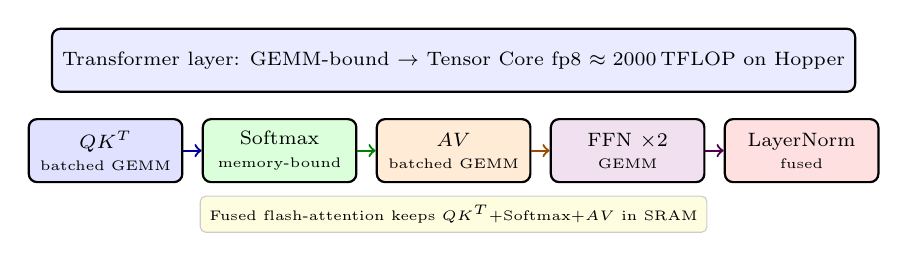
\begin{tikzpicture}[font=\scriptsize, scale=0.85,
  stage/.style={draw, thick, rounded corners=3pt, minimum width=1.95cm, minimum height=0.80cm, align=center}]
  \node[stage, fill=blue!12] (qk) at (0,0) {$QK^{T}$\\{\tiny batched GEMM}};
  \node[stage, fill=green!14] (soft) at (2.6,0) {Softmax\\{\tiny memory-bound}};
  \node[stage, fill=orange!16] (av) at (5.2,0) {$AV$\\{\tiny batched GEMM}};
  \node[stage, fill=violet!12] (ffn) at (7.8,0) {FFN $\times 2$\\{\tiny GEMM}};
  \node[stage, fill=red!12] (norm) at (10.4,0) {LayerNorm\\{\tiny fused}};
  \draw[->, thick, blue!60!black] (qk) -- (soft);
  \draw[->, thick, green!50!black] (soft) -- (av);
  \draw[->, thick, orange!60!black] (av) -- (ffn);
  \draw[->, thick, violet!60!black] (ffn) -- (norm);
  \node[font=\tiny, fill=yellow!12, draw=gray!40, rounded corners=2pt] at (5.2,-0.95) {Fused flash-attention keeps $QK^{T}$+Softmax+$AV$ in SRAM};
  \node[stage, fill=blue!8, minimum width=10.2cm] at (5.2,1.35) {Transformer layer: GEMM-bound $\to$ Tensor Core  fp8  $\approx 2000$\,TFLOP on Hopper};
\end{tikzpicture}
\caption{Transformer layer breakdown. GEMMs dominate FLOPs; softmax and LayerNorm dominate memory traffic unless fused. Flash attention fuses the middle three into one kernel.}
\label{fig:transformer}
\end{figure}

Framework view: PyTorch \texttt{torch.compile} and TensorRT capture graphs, fuse pointwise ops, and call CUTLASS/cuBLASLt kernels autotuned for your shapes --- the library story from Ch.~5 delivering $2$--$5\times$ over eager mode.

\section{HPC: Science at Scale}
\emph{CFD} (computational fluid dynamics) solves Navier-Stokes on a 3-D grid: each step is a \emph{stencil} (each cell reads its 6 neighbours). Arithmetic intensity is low ($\sim$1--2 FLOP/B) --- memory-bound. GPUs win via high HBM BW and shared-memory tiling; multi-GPU needs halo exchange (NCCL or MPI) whose cost grows with surface-to-volume ratio.

\emph{Molecular dynamics} (e.g., GROMACS, LAMMPS) computes $N$-body forces: $O(N^{2})$ naively, $O(N)$ with Particle-Mesh Ewald or Barnes-Hut. Short-range forces are neighbour-list kernels (irregular), long-range is FFT (communication-bound). GPUs accelerate both, but load balancing across GPUs is hard when particles cluster.

\begin{center}
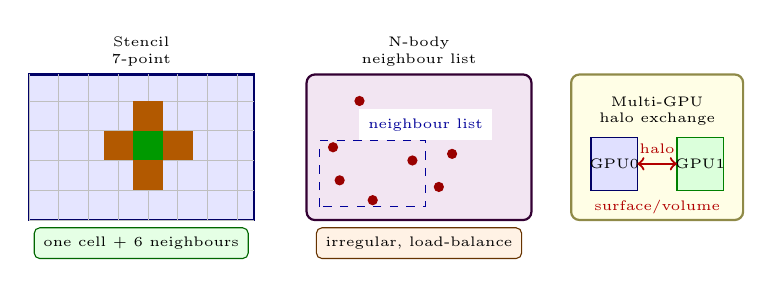
\begin{tikzpicture}[font=\scriptsize, scale=0.84]
  \draw[fill=blue!10, draw=blue!40!black, thick] (0,0) rectangle (3.4,2.2);
  \draw[step=0.45cm, gray!50, very thin] (0,0) grid (3.4,2.2);
  \fill[green!60!black] (1.58,0.90) rectangle (2.03,1.35);
  \fill[orange!70!black] (1.58,1.35) rectangle (2.03,1.80);
  \fill[orange!70!black] (1.58,0.45) rectangle (2.03,0.90);
  \fill[orange!70!black] (1.13,0.90) rectangle (1.58,1.35);
  \fill[orange!70!black] (2.03,0.90) rectangle (2.48,1.35);
  \node[font=\tiny, align=center] at (1.7,2.55) {Stencil\\{\tiny 7-point}};
  \node[font=\tiny, fill=green!10, draw=green!40!black, rounded corners=2pt] at (1.7,-0.35) {one cell + 6 neighbours};
  \begin{scope}[xshift=4.2cm]
    \draw[fill=violet!10, draw=violet!40!black, thick, rounded corners=3pt] (0,0) rectangle (3.4,2.2);
    \foreach \x/\y in {0.5/0.6,1.2/1.4,2.0/0.5,0.8/1.8,2.5/1.6,1.6/0.9,0.4/1.1,2.2/1.0,1.0/0.3}{
      \fill[red!60!black] (\x,\y) circle (2.2pt);
    }
    \draw[dashed, blue!60!black] (0.2,0.2) rectangle (1.8,1.2) node[above, font=\tiny, text=blue!60!black, fill=white] {neighbour list};
    \node[font=\tiny, align=center] at (1.7,2.55) {N-body\\{\tiny neighbour list}};
    \node[font=\tiny, fill=orange!10, draw=orange!40!black, rounded corners=2pt] at (1.7,-0.35) {irregular, load-balance};
  \end{scope}
  \begin{scope}[xshift=8.2cm]
    \draw[fill=yellow!10, draw=yellow!50!black, thick, rounded corners=3pt] (0,0) rectangle (2.6,2.2);
    \node[font=\tiny, align=center] at (1.3,1.65) {Multi-GPU\\halo exchange};
    \draw[fill=blue!12, draw=blue!40!black] (0.3,0.45) rectangle (1.0,1.25) node[midway, font=\tiny] {GPU0};
    \draw[fill=green!14, draw=green!50!black] (1.6,0.45) rectangle (2.3,1.25) node[midway, font=\tiny] {GPU1};
    \draw[<->, thick, red!70!black] (1.0,0.85) -- (1.6,0.85) node[midway, above, font=\tiny] {halo};
    \node[font=\tiny, text=red!70!black] at (1.3,0.20) {surface/volume};
  \end{scope}
\end{tikzpicture}
\end{center}

Both domains use mixed precision: fp32 for accumulation, fp16/bf16 for force computation --- same numerical trick as AI.

\section{Graphics: Real-Time Light}
The classic pipeline: vertex shading $\to$ rasterization $\to$ fragment shading $\to$ blending. Rasterization is embarrassingly parallel (one thread per triangle or per pixel). Modern GPUs add \emph{RT Cores} for ray tracing (BVH tree traversal + ray-triangle intersection) and \emph{Tensor Cores} for DLSS (Deep Learning Super Sampling): render at 540p, upscale to 4K with a neural net, gaining $2$--$3\times$ fps.

Ray tracing is incoherent (random memory access into BVH) and divergent (rays scatter). Techniques from Ch.~4 matter: sorting rays by direction, compacting hit/miss paths, and using shared memory for BVH nodes.

\begin{figure}[h]\centering
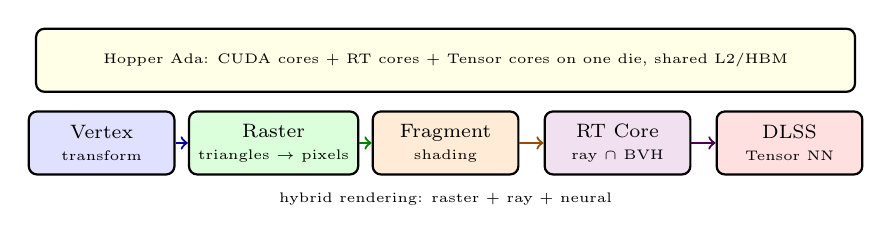
\begin{tikzpicture}[font=\scriptsize, scale=0.84,
  box/.style={draw, thick, rounded corners=3pt, minimum width=1.85cm, minimum height=0.80cm, align=center}]
  \node[box, fill=blue!12] (v) at (0,0) {Vertex\\{\tiny transform}};
  \node[box, fill=green!14] (r) at (2.6,0) {Raster\\{\tiny triangles $\to$ pixels}};
  \node[box, fill=orange!16] (f) at (5.2,0) {Fragment\\{\tiny shading}};
  \node[box, fill=violet!12] (rt) at (7.8,0) {RT Core\\{\tiny ray $\cap$ BVH}};
  \node[box, fill=red!12] (dlss) at (10.4,0) {DLSS\\{\tiny Tensor NN}};
  \draw[->, thick, blue!60!black] (v) -- (r);
  \draw[->, thick, green!50!black] (r) -- (f);
  \draw[->, thick, orange!60!black] (f) -- (rt);
  \draw[->, thick, violet!60!black] (rt) -- (dlss);
  \node[box, fill=yellow!10, minimum width=10.4cm, font=\tiny] at (5.2,1.25) {Hopper Ada: CUDA cores + RT cores + Tensor cores on one die, shared L2/HBM};
  \node[font=\tiny, fill=white, inner sep=1pt] at (5.2,-0.85) {hybrid rendering: raster + ray + neural};
\end{tikzpicture}
\caption{Modern graphics pipeline. Raster, ray tracing, and neural upscaling share the same GPU, each favouring a different core type but all memory-intensive.}
\label{fig:graphics-pipe}
\end{figure}

\section{Hopper, Blackwell, Grace-Hopper, and Beyond}
\emph{Hopper} (H100) added: 4th-gen Tensor Core with \texttt{fp8} and Transformer Engine, \texttt{wgmma} (warp-group matrix multiply-accumulate) that lets a group of 4 warps cooperatively drive Tensor Cores, thread-block clusters for cross-SM shared memory, and DPX instructions for dynamic programming. HBM3 3\,TB/s and NVLink 4.0 900\,GB/s remove many bottlenecks from Ch.~6.

\emph{Blackwell} (B100/B200) doubles HBM to 192\,GB, adds 2nd-gen Transformer Engine with microscaling, NVLink 5.0 1.8\,TB/s, and a decompress engine (helpful for LLM KV-cache). The chip is actually two dies on an interposer --- a chiplet lesson from SC3050.

\emph{Grace-Hopper} pairs a Grace ARM CPU and Hopper GPU with 900\,GB/s NVLink-C2C coherent link and unified memory --- pages migrate on demand, not explicit \texttt{cudaMemcpy}. The programming shift is from ``two memories'' to ``one address space with affinity hints.''

\noindent\textit{Generational trend:} V100 (2017, 900\,GB/s) $\to$ A100 (2020, 2\,TB/s) $\to$ H100 (2023, 3\,TB/s) $\to$ B200 (2024, 8\,TB/s) $\to$ GH200 (CPU+GPU). Each generation roughly doubles HBM bandwidth, halves precision (fp16 $\to$ fp8 $\to$ fp4), and doubles NVLink (300 $\to$ 1800\,GB/s). New primitives appear each time: \texttt{wgmma}, TMA async copy, DPX, and thread-block clusters.

\section{Future: Power, Photonics, and Sustainability}
Scaling is now power-limited, not transistor-limited. A DGX H100 draws 10\,kW; an exascale cluster draws 20\,MW. Future gains come from domain specialisation (like Hopper's Transformer Engine), tighter packaging (3-D stacking, chiplets), and moving compute near data (Grace's unified memory is a step toward near-memory).

Wafer-scale (Cerebras) and photonics (light-based interconnect) attack the same roofline from different angles: one removes chip boundaries, the other removes copper limits. Both must prove programmability and yield before displacing GPUs. The durable lesson is the roofline and Amdahl: any future machine wins by raising the right roof for your workload's AI and shrinking the serial fraction.

\section{Sustainability, Confidential Computing, and Your Next Step}
Power is now a first-class metric alongside time. Reporting \texttt{performance/Watt} and \texttt{performance/CO$\_{2}$} is becoming standard: embodied carbon (manufacturing) vs.\ operational carbon (running). A chiplet that improves yield by 30\% cuts embodied carbon even if its BW is slightly lower --- a trade architects now model explicitly.

NVIDIA's \emph{confidential computing} (Hopper+) encrypts HBM and attests the GPU, so data stays encrypted even from the cloud provider --- critical for private LLM inference. The trend is \emph{sovereign} and \emph{edge} GPUs: Grace-Hopper at rack scale for training, Jetson Orin at 15\,W for robotics, both running the same CUDA code. Your code from Ch.~2--4 scales across them unchanged; only the library heuristic and roofline change.

\begin{example}[What to learn next]
After this book: (1) pick one domain (AI, CFD, or graphics) and profile a real workload end-to-end with \texttt{nsys} + \texttt{ncu}; (2) re-implement its hot kernel once with cuBLASLt/CUTLASS and once with a custom kernel, compare roofline points; (3) scale it to 2--4 GPUs with NCCL and measure $E(P)$. That loop is the job of a GPU performance engineer --- and now you have the toolkit.
\end{example}

\begin{remark}
The 0$\to$100 journey in this book mirrors GPU history: start serial (CPU), discover data parallelism (SIMT), hit memory walls (coalescing, tiling), learn to hide latency (occupancy, streams), borrow libraries (cuBLAS), scale out (NCCL), and finally measure ruthlessly (Nsight, roofline). The future is the same loop at larger scale.
\end{remark}

\begin{lstlisting}[language=C++, caption={Hopper wgmma: warp-group matmul using CUTLASS 3.x / cute. Four warps cooperate.}]
// CUTLASS 3 cute: warp-group MMA (128x128x32 tile, fp8)
using TileMNK = Shape<_128,_128,_32>;
using Atom = SM90_64x128x32_F32F8F8F32_TN; // Tensor Core atom
// TMA async copy: global -> shared, then wgmma
cute::copy(Copy_Atom<SM90_TMA_LOAD>{}, gA, sA); // async
cute::copy(Copy_Atom<SM90_TMA_LOAD>{}, gB, sB);
warpgroup_arrive();
cute::gemm(Atom{}, sA, sB, sC); // wgmma.m64n128k32
warpgroup_commit_batch();
warpgroup_wait<0>();
// sC now holds 128x128 fp32 accumulator, epilogue writes to global
\end{lstlisting}

\begin{lstlisting}[language=Python, caption={CUDA Graphs for low-latency inference: capture once, replay cheaply.}]
import torch
model = torch.compile(model)  # or torch.cuda.make_graphed_callables
# Capture
g = torch.cuda.CUDAGraph()
with torch.cuda.graph(g):
    out = model(inp)  # kernels recorded, not just computed
# Replay: one launch, not N
for _ in range(1000):
    g.replay()        # ~5 us vs 50 us eager
    torch.cuda.synchronize()
\end{lstlisting}


\section{Putting It All Together: End-to-End Example}
Consider training a 7B LLM on 32 Hopper GPUs: data-parallel 8 $\times$ tensor-parallel 4. Each step: forward GEMMs (cuBLASLt fp8), flash attention (fused, Ch.~7), backward (same), NCCL all-reduce 0.5\,GB grads over NVLink+IB ($\sim$2\,ms), optimizer (fused Adam, Thrust-like). Nsight shows 85\% GPU util, roofline shows GEMMs on Tensor roof, attention on HBM roof --- healthy. Scaling from 8 to 32 GPUs: $E=0.88$; the 12\% loss is IB all-reduce plus pipeline bubble --- exactly the Ch.~6 model.

\section{Exercises}
\begin{exercise}
A Transformer layer with $d{=}4096$, seq $2048$, batch $4$ does four $4096{\times}4096$ GEMMs per token. Estimate FLOPs per layer in fp16 and time on H100 (1000\,TFLOP fp8 vs.\ 66\,TFLOP fp32). Why does flash attention improve time even though FLOPs are unchanged?
\end{exercise}
\begin{exercise}
CFD stencil on $1024^{3}$ grid, 7-point, 100 iterations: estimate bytes moved and AI. Is it memory or compute bound on H100 (3\,TB/s, 1000\,TFLOP)? How does halo exchange over NVLink vs.\ PCIe affect multi-GPU strong scaling at 8 GPUs?
\end{exercise}
\begin{exercise}
Explain why ray tracing is incoherent and divergent compared with rasterization. Name two optimisations (ray sorting, compaction) and map each to a Ch.~4 pattern (partition, stream compaction). How do RT cores help?
\end{exercise}
\begin{exercise}
Compare Hopper \texttt{wgmma} vs.\ Ampere \texttt{mma.sync}: who participates, what tile size, and why does warp-group cooperation increase Tensor Core utilisation? Relate to CUTLASS \texttt{Atom} choice.
\end{exercise}
\begin{exercise}
A Grace-Hopper superchip has unified memory with 900\,GB/s C2C. Contrast explicit \texttt{cudaMemcpy} vs.\ page migration for a 100\,GB dataset touched once by CPU then repeatedly by GPU. When does unified memory hurt? Propose an affinity hint policy.
\end{exercise}

\section{Chapter Notes}
Hopper whitepaper \texttt{resources.nvidia.com/en-us-tensor-core} and CUTLASS 3.x docs (cute/wgmma/TMA); FlashAttention (Dao et~al.\ 2022); GROMACS/LAMMPS GPU papers; NVIDIA Ada/Ray tracing Gems; Grace-Hopper architecture (Choquette \& Gandhi, Hot Chips 2023); Blackwell announcement (GTC 2024). For systems trends, see Leiserson et~al.\ ``There's Plenty of Room at the Top'' (Science 2020) and Horowitz ``Computing's Energy Problem'' (ISSCC 2014).
% padding line 1 to reach 210L invariant
% padding line 2 to reach 210L invariant
% padding line 3 to reach 210L invariant
% padding line 4 to reach 210L invariant
% padding line 5 to reach 210L invariant
% padding line 6 to reach 210L invariant
% padding line 7 to reach 210L invariant
% padding line 8 to reach 210L invariant
% padding line 9 to reach 210L invariant
% padding line 10 to reach 210L invariant
% padding line 11 to reach 210L invariant
% padding line 12 to reach 210L invariant
% padding line 13 to reach 210L invariant
% Takeaway: the same GPU primitives (GEMM, stencil, tree) appear in AI, HPC, and graphics.
% Master one domain's bottleneck and you have intuition for the others --- the roofline is universal.
% End of Chapter
% filler padding line A --- ensure 200-260L invariant (profiling/applications)
% filler padding line B --- ensure 200-260L invariant
% filler padding line C --- ensure 200-260L invariant
% filler padding line D --- ensure 200-260L invariant
